\begin{frame}
  \begin{block}{Características}
    \begin{itemize}
      \item Pontos de acesso de baixos alcance, custo, consumo de energia
      \item \textit{aka \alert{home base-stations}}
      \item Ajudam a melhorar a cobertua em pequenas áreas%, conectando
      %localmente redes celulares e roteando o tráfego através da Internet
      \item \textit{Bridge} entre o usuário e a rede da operadora usando a
      Internet
    \end{itemize}
  \end{block}
	\begin{figure}[!htb]
		\centering
		\subfloat[Femtocell]{
			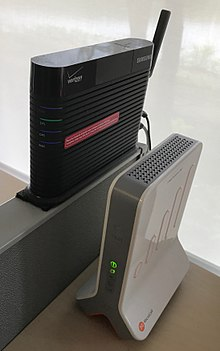
\includegraphics[height=3.5cm]{./Figures/Femtocell}
			\label{figdroopy}}
		\quad %espaco separador
		\subfloat[Macrocells]{
			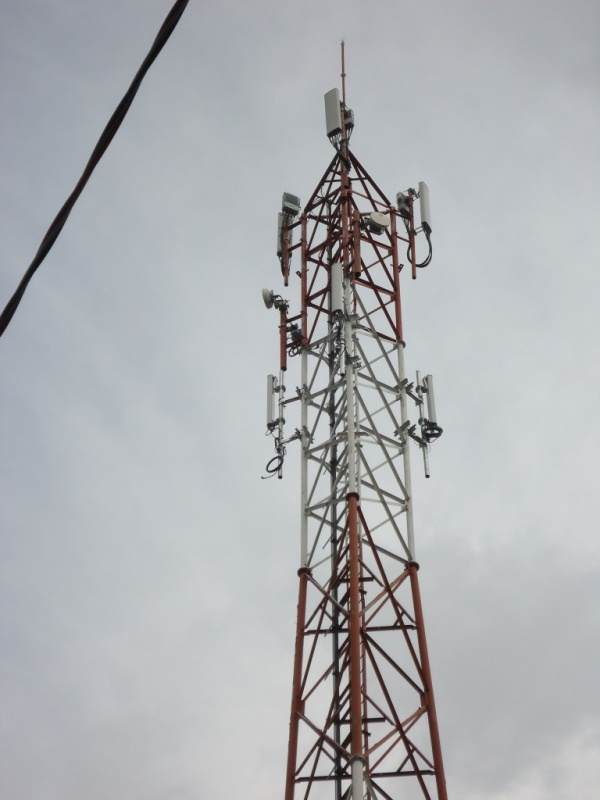
\includegraphics[height=3.5cm]{./Figures/Macrocell}
			\label{figsnoop}
			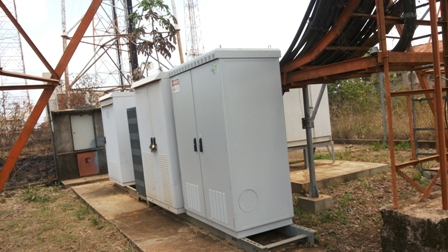
\includegraphics[height=2.5cm]{./Figures/Macrocell2}
			\label{figsnoop}}
		%\caption{Subfiguras}
		%\label{fig01}
	\end{figure}
\end{frame}

\begin{frame}
  \begin{figure}[h]
  	\begin{center}
      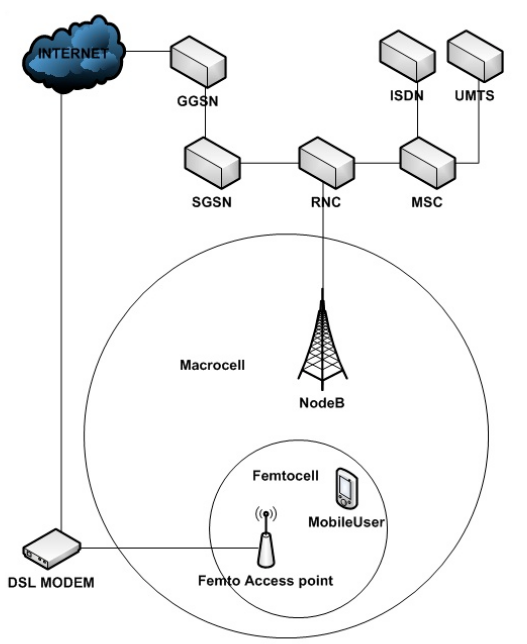
\includegraphics [scale=0.35]{./Figures/FemtocellTopology}
      \caption {Cenário Típico de utilização de \textit{Famtomcells}
      \cite{green-markov}.}
  		\label{fig:FemtocellTopology}
  	\end{center}
  \end{figure}
\end{frame}

\begin{frame}
  \begin{block}{Vantagens}
    \begin{itemize}
      \item Melhor cobertura de sinal (ambientes de difícil acesso, ambientes
      \textit{indoor}, etc...)
      \item Tipicamente instalados por não-especialistas
      \item Auto-organização dos parâmetros operacionais
      \item Cliente se associa automaticamente a \textit{femtocell} de melhor
      potência de sinal
    \end{itemize}
  \end{block}

  \begin{block}{Desvantagens da associação por potência de sinal}
    \begin{itemize}
      \item Possibilidade de sobrecarga de células
      \item Mau balanceamento de clientes entre células
      \item A escolha pode não atender critérios de QoS demandadas pela
      aplicação
    \end{itemize}
  \end{block}
\end{frame}

%\begin{frame}
%  \begin{block}{}
%    \begin{itemize}
%      \item
%    \end{itemize}
%  \end{block}
%\end{frame}

%\begin{frame}
%  \begin{block}{}
%  \end{block}
%\end{frame}

%\begin{frame}
%  \begin{figure}[h]
%  	\begin{center}
%      \includegraphics [scale=0.3]{./Figures/Device-Estimates}
%     % \caption {Estimativa de dispositivos conectados à Internet.}
%  		%\label{fig:arq-imuno}
%  	\end{center}
%  \end{figure}
%\end{frame}

%\begin{frame}{Redes de Acesso}
%	\begin{figure}[!htb]
%		\centering
%		\subfloat[DSL]{
%			\includegraphics[height=3.5cm]{./Figures/DSLaccess}
%			\label{figdroopy}}
%		\quad %espaco separador
%		\subfloat[Cable]{
%			\includegraphics[height=3.5cm]{./Figures/CableAccess}
%			\label{figsnoop}}
%		%\caption{Subfiguras}
%		%\label{fig01}
%	\end{figure}
%\end{frame}

%\begin{frame}[fragile]
%\scriptsize
%\begin{verbatim}
%\end{verbatim}
%\end{frame}
